\chapter{Métodos y recursos}
\label{chapter:Métodos y recursos}


\section{Introducción}

Este capítulo presenta la metodología y las herramientas empleada en el desarrollo del proyecto, detallando cada fase de diseño, implementación y pruebas. 
Tras realizar una planificación exhaustiva y un análisis del estado del arte en el capítulo anterior, se ha adquirido un marco preciso sobre los objetivos y las etapas necesarias para alcanzar los objetivos de este proyecto. 
Con esta base sólida, se procede a estructurar y ejecutar el desarrollo del producto utilizando metodologías y recursos que se ajusten a las necesidades de automatización y procesamiento de datos que plantea el proyecto.

\subsection{Descripción general del capítulo}

El capítulo muestra un desglose de las decisiones metodológicas y técnicas que sustentan el diseño y desarrollo de la solución. 
Incluye una descripción de los recursos tecnológicos, tanto de hardware como de software, empleados para asegurar la eficiencia y precisión en el proceso de identificación y clasificación de convocatorias de ayudas. 
Cada sección aborda de manera específica las técnicas y herramientas implementadas en cada fase del proyecto, desde la recopilación de datos con el extractor de ayudas, la generación de datos estructurados con el bloque de procesamiento, y la construcción de la herramienta de consulta de información basada en un sistema conversacional basado en agentes inteligentes.

\subsection{Importancia del diseño, desarrollo e implementación en la investigación}

El desarrollo de una solución automatizada para sintetizar y recuperar información de convocatorias es esencial en un entorno con abundancia de datos y formatos diversos. 
Un diseño eficiente asegura que cada componente cumpla su función, maximizando la precisión y minimizando redundancias. 
La implementación adapta técnicas de recuperación de información y procesamiento de lenguaje natural basadas en Inteligencia Artificial Generativa, del estado del arte a las necesidades del proyecto, mientras que una metodología ágil permite ajustes continuos y mejora constante.
Este capítulo describe los métodos y recursos que sustentan la construcción de la solución, transformando la planificación teórica en un producto funcional capaz de procesar grandes volúmenes de datos y facilitar su análisis para entidades específicas.

\section{Objetivos y Competencias}

El propósito de esta sección es detallar los objetivos específicos de la fase de desarrollo e implementación de la solución, y las competencias técnicas y metodológicas necesarias para cumplir con dichos objetivos. 
Estos aspectos son fundamentales para asegurar que cada etapa del proyecto esté alineada con los resultados esperados y que los participantes en el desarrollo cuenten con las habilidades necesarias para abordar los desafíos que puedan surgir.


\subsection{Objetivos específicos de esta fase del proyecto}

Los objetivos de la fase de desarrollo e implementación son los siguientes:

\begin{itemize}
    \item \textbf{Implementación de un sistema automático de extracción de datos de ayudas}: 
    Desarrollo de una herramienta basada en web scraping para la extracción de información.
    Esta herramienta es modular, cada uno de estos módulos está adaptadoa una fuente de convocatorias específica.
    La herramienta navega por el sitio web, identifica las diferentes convocatorias disponibles y extrae la información necesaria, como el texto resumen de la ayuda, la ficha técnica, y los documentos asociados a la convocatoria.
    \item \textbf{Desarrollo de un módulo de procesamiento de datos}: 
    Este módulo carga las fuentes de datos asociadas a cada ayuda y las procesa mediante técnicas de extracción basadas en IA Generativa.
    El objetivo es extraer diferentes parámetros de las fuentes de datos y obtener como resultado un conjunto de datos estructurados en formato tabla.
    \item \textbf{Desarrollo de un módulo de construcción de bases de datos}:
    Este módulo parte de las fuentes de datos originales y de los datos estructurados y contruye una base de datos documental y una base de datos estructurados.
    Mientras que en este caso, la base de datos estructural se crea de manera directa, para la base de datos documental es necesario implemental un bloque de procesamiento, donde los diferentes documentos se dividen en chunks y se generan sus correspondientes embeddings.
    \item \textbf{Implementación de una aplicación RAG mediante técnicas avanzadas}:
    Construcción de una solución de recuperación de información basada en un RAG multiagente, donde a través de lenguaje natural pueden generarse consultas de datos tanto a la base de datos estructurada como a la documental.
    \item \textbf{Implementación de una aplicación web para el uso del sistema multiagente como asistente conversacional}:
    Construcción de una pequeña interfaz de chat para la explotación de la herramienta de recuperación de información.
\end{itemize}

Estos objetivos son claves para asegurar que el sistema cumpla con los requisitos del proyecto y
proporcione una herramienta robusta y confiable para la identificación y análisis de convocatorias de
ayudas.



\subsection{Competencias técnicas y metodológicas requeridas}

Para la implementación de la solución de este proyecto, es necesario estar capacitado en una serie de competencias técnicas, tanto en el ámbito del desarrollo de software como en relación a diferentes técnicas de Inteligencia Artificial Generativa, Agentes inteligentes y frameworks específicos.

\begin{itemize}
    \item \textbf{Desarrollo de sistemas de captura de datos basados en web scraping}:
    Se requiere conocimiento y experiencia en herramientas y frameworks de scraping para la extracción de datos en multiples entornos web, como son el caso de BeautifulSoup y Selenium.

    \item \textbf{Desarrollo de sistemas de procesamiento de datos}:
    Conocimiento en implementación de pipelines de extracción, transformación y carga de datos. 
    Conocimiento de las principales herramientas de tratamiento de datos dentro del ecosistema Python (Numpy, Pandas, sqlalchemy).
    
    \item \textbf{Implementación de sistemas basados en Inteligencia Artificial Generativa}:
    Es necesaria una base de Procesamiento de Lenguaje Natural, que permita entender el funcionamiento de los Grandes Modelos del Lenguaje y las diferentes aplicaciones que se pueden construir con éstos.
    Se requiere, además, conocimiento de las diferentes opciones a emplear en cuanto a modelos del lenguaje, arquitecturas de uso, y vectorización de texto mediante embeddings (Prompt engineering, Retrieval Augmented Generation, Data Extraction, etc).
    
    \item \textbf{Frameworks de orquestación de soluciones basadas en LLMs y Agentes Inteligentes}: 
    Partiendo del punto anterior, es necesario el uso de frameworks específicos de IA generativa, los cuales permiten simplificar y normalizar el uso de estas herramientas. 
    Frameworks como LangChain y LanGpraph permiten implementar soluciones estandarizadas y funcionales con cualquier tipo de arquitectura, desde fuentes de datos a uso de diferentes modelos del lenguaje.
    También permiten la construcción de grafos de procesamiento donde se pueden implementar diferentes agentes, cada uno con una función específica. 
    
    \item \textbf{Bases de datos relacionales y vectoriales}: 
    Se requiere conocimientos en diseño y gestión de bases de datos relacionales para el almacenamiento y la información estructurada generada por el sistema.
    Así mismo, se requieren conocimientos en bases de datos vectoriales (FAISS, Choma, etc) para el almacenamiento y consulta de los diferentes documentos, y sus embeddings asociados.

    \item \textbf{Implementación de interfaz gráfica}: 
    Capacidad para implementar una interfaz gráfica que permita el uso de la aplicación mas allá de una consola de comandos.   
\end{itemize}

Estas competencias son fundamentales para abordar los objetivos de este proyecto, y obtener como resultado un sistema robusto y eficiente que sea capaz de cumplir las necesidades establecidas. 


\section{Diseño del sistema}

La solución desarrollada está estructurada en tres bloques principales: El sistema de extracción, el módulo de procesamiento, y la aplicación de consulta.
Estos tres módulos trabajan en conjunto para formar un sistema automatizable que extraiga información a partir de diferentes fuentes de convocatorias, las procese debidamente, y las incluya en el asistente conversacional de consulta.

\subsection{Arquitectura general}

La arquitectura general del sistema se compone de los siguientes módulos principales:

\begin{itemize}
    \item \textbf{Módulo de Extracción de Datos}:
    La principal funcionalidad de este módulo es la búsqueda, en cada uno de los portales de convocatorias incluidos en el sistema, de diferentes convocatorias de ayudas disponibles.
    Para cada ayuda encontrada, el sistema identifica diferentes fuentes de datos necesarias: Texto resumen de la convocatoria, ficha técnica, y documentos (generalmente pdf) asociados a la convocatoria o a sus bases.
    Este módulo se basa principalmente en herramientas de web scraping, específicamente BeautifulSoup para la intepretación de código HTML, y Selenium para la navegación por sitios web dinámicos.
    Además de la extracción, también implementa una pequeña sección de preprocesamiento, para construir diferentes documentos de formato markdown para el texto plano extraido del sitio web, así como la descarga correcta de los documentos pdf, y la organización de estos documentos.

    \item \textbf{Módulo de Procesamiento de Datos}:
    Este módulo implementa un flujo de procesamiento basado en técnicas de procesmaiento de datos estandar, combinadas con técnicas basadas en IA generativa para la extracción de un conjunto de parámetros específicos para cada ayuda.
    Internamente se han empleado diferentes técnicas implementadas desde el framework LangChain: Prompt Engineering para la construcción de prompts robustos de extracción de datos, cadenas de procesamiento de LangChain para la implementación de pipelines, y técnicas de RAG para la extracción de información de documentos mas extensos.
    
    \item \textbf{Módulo de Construcción de Bases de Datos}:
    Este módulo parte de los datos de convocatorias en crudo y de los datos estructurados extraidos del módulo anterior, y los integra en las diferentes bases de datos del sistema.
    En este caso, la integración de los datos estructurados se realiza en una base de datos SQL, mientras que los documentos pasan por un proceso de segmentación en chunks, generación de embeddings y integración en una base de datos vectorial.

    \item \textbf{Sistema de Recuperación de Información (RAG multiagente)}:
    Esta aplicación consiste en una arquitectura RAG multiagente avanzada, donde dispone de la base de datos vectorial y la base de datos SQL como fuentes documentales, a las cuales puede acceder, realizar búsquedas y extraer información contextual en base a las consultas realizadas.
    Está construida desde los frameworks LangChain y LanGraph y permite enlazar un Gran Modelo del Lenguaje a las fuentes de datos.
    \item \textbf{Interfaz de Usuario}:
    Se ha desarrollado una interfaz de usuario sencilla empleando la librería Streamlit, la cual permite levantar en pocas líneas de código una aplicación gráfica a modo de chatbot, e interactuar con el RAG multiagente.
\end{itemize}



\subsection{Flujo de trabajo del sistema}

La solución planteada está diseñada para que se pueda ejecutar de forma eficiente siguiendo un flujo de trabajo, integrando todo el proceso ETL que supone la búsqueda de convocatorias con la herramienta de consulta.
Los pasos clave del flujo de trabajo son los siguientes:

\begin{itemize}
    \item \textbf{Extracción de datos}:
    El módulo de extracción emplea web scraping para la búsqueda y descarga de las diferentes ayudas encontradas, siguiendo un algoritmo de búsqueda específico para cada portal de ayudas, ya que éste está ligado al formato de la página web.

    \item \textbf{Procesamiento de datos}:
    A partir de los datos en crudo se generan dos flujos de trabajo: El primero consiste en la extracción de parámetros y variables específicas de las fuentes de cada ayuda, mientras que el segundo realiza un preprocesado de los documentos, los divide en chunks y genera sus embeddings asociados.

    \item \textbf{Carga en las bases de datos}: A partir de los datos procesados, se actualizan tanto la base de datos SQL como la vectorial, además de generar los ficheros binarios necesarios para la aplicación RAG.

    \item \textbf{Integración de la aplicación RAG con las bases de datos}:
    Una vez han sido actualizadas las bases de datos, la aplicación RAG ya tiene acceso al contenido actualizado.
\end{itemize}

La solución está planteada de forma que se ejecuten periódicamente los tres primeros pasos para mantener actualizadas las bases de datos.


\section{Tecnologías y herramientas}

En esta sección se describen las herramientas y tecnologías seleccionadas para la implementación del sistema y el desarrollo de cada módulo.
Las tecnologías empleadas han sido seleccionadas en base a su eficacia, su posición dentro de cada grupo de tecnologías específicas que se emplean en el mercado, y su facilidad para implementar en un entorno local con pocos recursos.


\subsection{Tecnologías seleccionadas}

A continuación, se detallan las tecnologías clave empleadas:

\begin{itemize}
    \item \textbf{Python}: Se ha seleccionado Python como lenguaje de desarrollo principal por razones obvias: Es el lenguaje de programación mas empleado en el campo de la Ciencia de Datos y la Inteligencia Artificial. Esto implica que la gran mayoría de herramientas, frameworks y librerías de estos ámbitos están disponibles en Python. Esto, junto a la simplicidad que presenta el propio lenguaje, facilita y simplifica el desarrollo de cualquier solución de esta índole.
    
    \item \textbf{Beautifulsoup y Selenium}: Para la extracción de datos de sitios web, se utilizan BeautifulSoup y Selenium. 
    BeautifulSoup permite analizar y manipular la estructura HTML de las páginas, mientras que Selenium se emplea para interactuar con sitios web que requieren carga dinámica de contenido. 
    Juntos, estos paquetes permiten implementar un sistema de extracción robusto, capaz de navegar y extraer información relevante de manera eficiente.
    
    \item \textbf{SQLite}: SQLite es un sistema de gestión de bases de datos relacional embebido, de código abierto, que implementa una base de datos transaccional autocontenida, sin necesidad de un servidor dedicado. 
    Se caracteriza por su ligereza, portabilidad y facilidad de integración en aplicaciones de escritorio, móviles y sistemas embebidos. 
    SQLite almacena los datos en un único archivo en disco, lo que simplifica la gestión y el despliegue, mientras que soporta operaciones ACID, garantizando la integridad y fiabilidad de los datos. 
    Su arquitectura libre de configuración lo convierte en una solución óptima para aplicaciones que requieren una base de datos local con bajo consumo de recursos y alta eficiencia en operaciones de lectura y escritura.
    
    \item \textbf{FAISS} (Facebook AI Similarity Search): es una librería de código abierto desarrollada por Meta AI, diseñada para realizar búsquedas eficientes de vectores de alta dimensión, optimizando la recuperación de similitudes en grandes volúmenes de datos. 
    FAISS permite construir índices que soportan tanto búsquedas exactas como aproximadas, utilizando técnicas avanzadas de cuantización y particionamiento, lo que la hace especialmente adecuada para aplicaciones de recuperación de información. 
    Gracias a su arquitectura optimizada para CPU y GPU, FAISS ofrece un alto rendimiento en tareas de búsqueda a gran escala, permitiendo gestionar millones o incluso miles de millones de vectores con tiempos de respuesta reducidos y consumo eficiente de recursos.
    
    \item \textbf{FAISS - BM25}: La extensión de FAISS para soporte de modelos de recuperación basados en términos, como BM25 (Best Matching 25), permite combinar las capacidades de búsqueda vectorial de alta dimensión con técnicas clásicas de recuperación de información basadas en el modelo probabilístico BM25. 
    Esta integración posibilita la indexación y búsqueda eficiente de documentos textuales, aplicando BM25 sobre representaciones de términos discretos mediante mecanismos optimizados dentro del entorno de FAISS. 
    De esta manera, se obtiene una solución híbrida que aprovecha la eficiencia y escalabilidad de FAISS para búsquedas aproximadas, al tiempo que incorpora un modelo estadístico robusto y ampliamente probado para la recuperación de documentos basada en la relevancia por frecuencia de término e inverso de frecuencia documental (TF-IDF mejorado). 
    Esta capacidad permite diseñar sistemas de búsqueda más versátiles y precisos en escenarios donde se requiere combinar búsquedas semánticas con búsquedas léxicas tradicionales.
    
    \item \textbf{LangChain}: Es un framework de código abierto orientado a la creación de aplicaciones que integra Grandes Modelos del Lenguaje con fuentes de datos externas, herramientas y flujos de trabajo complejos. 
    Su arquitectura modular permite orquestar cadenas de llamadas a modelos, agentes, memorias y herramientas externas, facilitando la construcción de aplicaciones conversacionales, asistentes virtuales, sistemas de pregunta-respuesta sobre documentos y soluciones de razonamiento avanzado. 
    LangChain proporciona abstracciones de alto nivel para gestionar la interacción dinámica entre modelos, usuarios y datos, soportando integraciones con bases de datos vectoriales, motores de búsqueda, APIs y sistemas de recuperación de información. 
    Esto permite desarrollar soluciones contextuales, reactivas y personalizadas que aprovechan el potencial de los LLMs combinándolos con lógica de negocio, flujos condicionales y datos propios de la organización.
    
    \item \textbf{LanGraph}: Es una extensión de código abierto para LangChain que permite modelar y ejecutar flujos conversacionales complejos mediante grafos de estado dinámicos. 
    Basado en el paradigma de máquinas de estado y grafos dirigidos, LangGraph proporciona una abstracción flexible para definir nodos que encapsulan agentes, cadenas de modelos de lenguaje, funciones o cualquier unidad lógica, permitiendo controlar de manera explícita las transiciones entre estados en función de la entrada, el contexto o condiciones personalizadas. 
    Esta capacidad resulta especialmente útil para construir aplicaciones conversacionales multi-turno, flujos de trabajo ramificados, agentes colaborativos y sistemas de toma de decisiones basados en LLMs. 
    Además, LangGraph permite la reutilización, trazabilidad y depuración de flujos, facilitando el desarrollo de sistemas robustos, auditables y adaptables a escenarios empresariales complejos donde se requiere control granular del comportamiento conversacional y de los procesos impulsados por inteligencia artificial.
    
    \item \textbf{Azure AI Studio}: Es una plataforma integrada dentro del ecosistema Microsoft Azure, orientada a facilitar el desarrollo, despliegue y gestión de aplicaciones basadas en inteligencia artificial generativa. 
    Proporciona un entorno unificado para construir soluciones personalizadas combinando modelos de lenguaje, visión, voz y decisiones, integrados con datos corporativos y flujos de negocio. 
    Azure AI Studio permite a las organizaciones acelerar el ciclo de vida de desarrollo de aplicaciones de IA generativa mediante herramientas visuales, asistentes guiados y flujos predefinidos, al tiempo que asegura la gobernanza, seguridad y cumplimiento normativo mediante políticas de Azure. 
    Además, ofrece capacidades avanzadas para la orquestación de flujos de trabajo de IA, integración con Azure OpenAI Service, Azure Machine Learning, y conectividad con fuentes de datos empresariales, permitiendo desarrollar soluciones escalables, seguras y adaptadas a necesidades específicas de negocio.

    Dentro de Azure AI Studio se han empleado los siguientes modelos:
    \begin{itemize}
        \item \textbf{o3-mini}: Es un modelo de razonamiento ligero y rentable optimizado para tareas de programación, matemáticas y ciencia, que ofrece tres niveles de esfuerzo de razonamiento (bajo, medio y alto) y soporta funcionalidades avanzadas como Structured Outputs y llamada de funciones.
        \item \textbf{text-embedding-3-large}: Es el modelo de incrustaciones de texto de siguiente generación de OpenAI, que genera vectores de hasta 3072 dimensiones para representar conceptos en texto y código.
    \end{itemize}

    \item \textbf{Streamlit}: Es un framework de código abierto orientado al desarrollo ágil de interfaces web interactivas para aplicaciones de ciencia de datos, machine learning y visualización de información. 
    Diseñado con un enfoque declarativo y minimalista, Streamlit permite a los desarrolladores crear aplicaciones web funcionales utilizando exclusivamente Python, sin necesidad de conocimientos avanzados en desarrollo frontend. 
    La plataforma facilita la integración directa con librerías populares como Pandas, Matplotlib, Plotly o TensorFlow, permitiendo desplegar dashboards interactivos, formularios y visualizaciones en tiempo real con mínima complejidad. 
    Además, Streamlit soporta actualizaciones reactivas y dinámicas del contenido en función de la interacción del usuario, habilitando la creación de prototipos rápidos, demostradores y herramientas de toma de decisiones basadas en datos de manera eficiente y escalable.
\end{itemize}



\subsection{Implementación del módulo de extracción de datos}

Este módulo ha sido el primero en desarrollarse, y su función principal es la búsqueda y recopilación de datos de plataformas en diversas plataformas.
Está diseñado con una arquitectura modular, en la cual se pueden integrar diferentes módulos asociados a cada fuente de convocatorias. 


\begin{itemize}
    \item \textbf{Fuentes de datos}: En principio, se ha implementado el módulo asociado a la plataforma CDTI, pudiendo integrarse diferentes módulos posteriormente.
    \item \textbf{Extracción de datos y documentos}: Para la extracción de datos intrínsecos de los sitios web, se emplea la combinación de BeautifulSoup con Selenium.
    Mientras que Beautifulsoup permite la busqueda y extracción de información a partir de las etiquetas HTML, Selenium permite interactuar con páginas que requieren carga dinámica, como botones, tablas, o bloques de texto cargados mediante Javascript.
    Adicionalmente, se identifican posibles enlaces a documentación en formato PDF.
    \item \textbf{Preprocesamiento de datos}: Para cada página asociada a una convocatoria, se extraen diferentes bloques de texto o datos, los cuales son sometidos  auna limpieza inicial, eliminando duplicados, normalizando el formato e integrando diferentes bloques para formar un documento de texto en formato Markdown.
\end{itemize}



\subsubsection{Implementación del módulo específico para CDTI}

El módulo asociado a CDTI sigue el siguiente flujo de trabajo:

\begin{itemize}
    \item En primer lugar se identifica la Matriz de ayudas. El portal web de CDTI presenta una tabla con diferentes ayudas disponibles según siferentes categorías. Como primer paso, el módulo extrae esa matriz de ayudas junto a los enlaces correspondientes.
    \item Para cada ayuda disponible en la matriz de ayudas, El módulo analiza su página principal, e identifica los siguientes elementos:
    \begin{itemize}
        \item Bloque de resumen de la ayuda.
        \item Ficha técnica.
        \item Enlaces a documentación.
        \item Posibles subpáginas.
    \end{itemize}
    \item En el caso que existan subpáginas, entra en ellas y repite el proceso de extracción.
    \item En el caso que existan enlaces a documentación, descarga el documento en el directorio local correspondiente mediante el comando Start-BitsTransfer de Powershell.
    Tras haber testeado diferentes métotos de descarga desde Python, esta ha sido la única solución desde Windows que permitía extraer el documento pdf correctamente. 
    \item Una vez identificados todos los bloques de texto necesarios, pasan por un preprocesado inicial para generar tres documentos en formato markdown:
    \begin{itemize}
        \item Description: Documento con el texto resumen y/o introductorio de la ayuda.
        \item Card: Ficha técnica de la ayuda.
        \item Metadata: Enlaces a documentación.
    \end{itemize}
\end{itemize}


\begin{figure}[h]
	\centering
	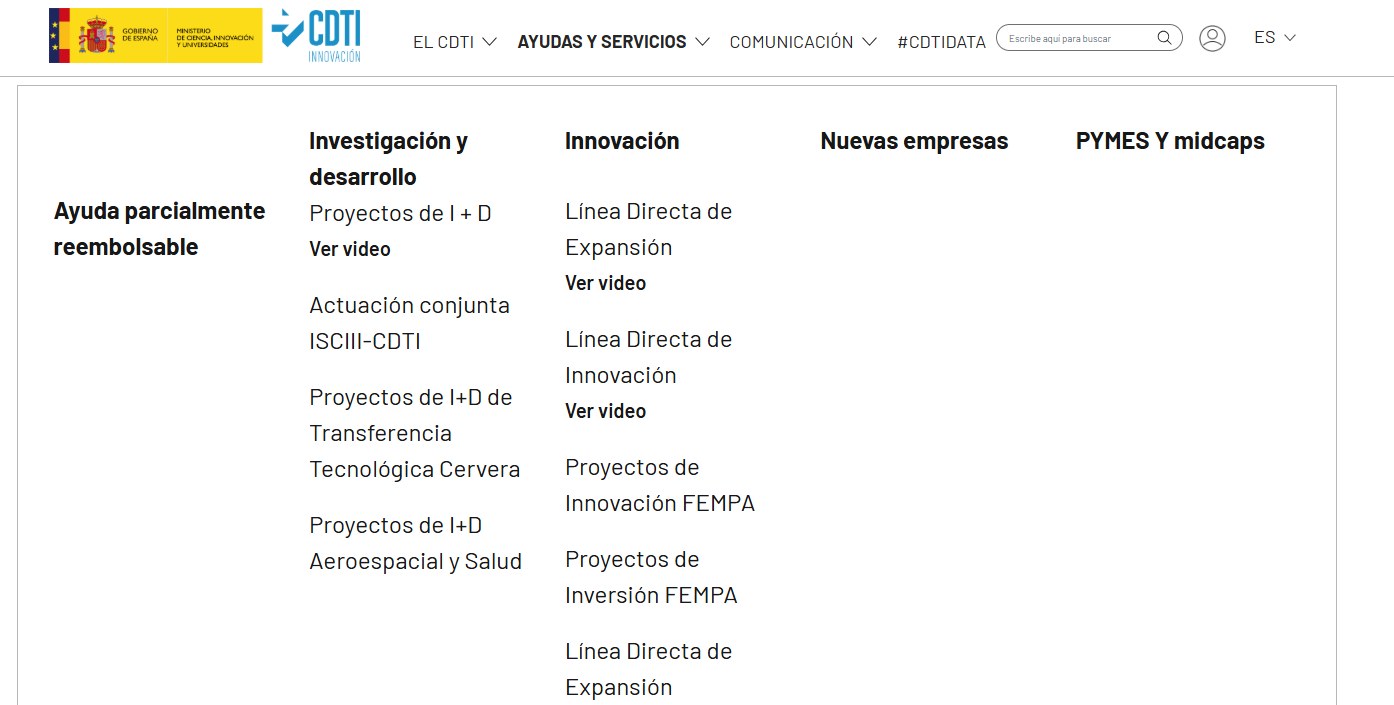
\includegraphics[width=0.8\textwidth]{figs/cdti_matrix.png}
	\caption{Matriz de ayudas del CDTI}
	\label{fig:context-anoni1}
\end{figure}


Tras la ejecución del módulo, obtenemos un directorio local para cada ayuda con los tres documentos markdown y los pdf asociados a la ayuda.

%meter esquema de codigo

\subsection{Implementación del módulo de procesamiento de datos}

La funcionalidad principal de éste módulo es la extracción de determinados valores o parámetros específicos de cada ayuda, con el objetivo de construir una base de datos estructurada con esa información.

Para ello, se ha diseñado una solución basada en IA Generativa que permite analizar los diferentes documentos asociado a la convocatoria de ayuda y extraer los siguientes parámetros:

\begin{itemize}
    \item \textbf{organismo}: Entidad que da la subvención.
    \item \textbf{nombre}: Título de la ayuda o subvención. 
    \item \textbf{linea}: Modalidades de la subvención.
    \item \textbf{fecha\_inicio}: Fecha de inicio del plazo para presentar la solicitud.
    \item \textbf{fecha\_fin}: Fecha de fin del plazo para presentar la solicitud.
    \item \textbf{objetivo}: Objetivo general de la ayuda o actuación.
    \item \textbf{beneficiarios}: Beneficiarios de la ayuda o actuación.
    \item \textbf{anio}: Año de la convocatoria.
    \item \textbf{area}: Clasificación de la ayuda en una de las siguientes áreas:I+D, Innovación, Inversión o Internacional.
    \item \textbf{presupuesto\_minimo}: Valor del presupuesto mínimo.
    \item \textbf{presupuesto\_maximo}: Valor del presupuesto máximo.
    \item \textbf{duración\_mínima}: Duración mínima de la ayuda.
    \item \textbf{duración\_máxima}: Duración máxima de la ayuda.
    \item \textbf{intensidad\_del\_prestamo}: Información sobre la intensidad del préstamo.
    \item \textbf{tipo\_financiacion}: Tipo de la ayuda.
    \item \textbf{link\_ficha\_tecnica}: URL de la página principal de la ayuda.
    \item \textbf{link\_convocatoria}: URL de los documentos PDF asociados a la ayuda.
\end{itemize}

De la misma manera que el módulo de extracción de datos, este módulo ha sido diseñado de forma que exista un submódulo asociado a cada portal de ayudas específico.
Esto es debido a que cada portal tiene su propia arquitectura y formato de distribución de la información. 
En el caso de CDTI, los datos a extraer se encuentran tanto en la ficha técnica como en el PDF de la convocatoria.


\subsubsection{Implementación del módulo específico para CDTI}

El módulo asociado a CDTI sigue el siguiente flujo de trabajo para cada ayuda:

\begin{itemize}
    \item Se cargan los documentos markdown como texto plano y se concatenan para tener un único documento. También se carga por otro lado el pdf a texto plano con el loader estándar de LangChain.
    \item Ese documento pasa por una cadena de LangChain con un prompt de extracción de un subconjunto de las variables anteriores. 
    La cadena genera directamente un JSON con las variables y su contenido.
    \item Por otro lado, se genera otra cadena con una arquitectura de "RAG dinámico" donde a partir de otro conjunto de prompts, se extrae el resto de variables, también en formato JSON. 
    \item Finalmente, se concatenan ambos JSON para tener el registro completo de la ayuda.
\end{itemize}

El módulo se ejecuta para cada una de las ayudas disponibles de CDTI, y finalmente se concatenan para construir un DataFrame de Pandas, el cual se almacena en local como fichero CSV.


\subsection{Implementación del módulo de construcción de las bases de datos}

La finalidad de este módulo es la carga de los datos obtenidos para cada ayuda al conjunto de bases de datos que conforman la solución.
Estas bases de datos son:

\begin{itemize}
    \item Una base de datos relacional, donde se almacena una la tabla \textbf{aids\_table}, con los campos previamente descritos para cada ayuda.
    \item Una base de datos vectorial, donde se almacenan los documentos pertinentes de cada una de las ayudas.
    \item Adicionalmente, se emplea un directorio local para almacenar ficheros binarios necesarios para la aplicación.
\end{itemize}

Aunque ya se ha realizado procesamiento de datos en el módulo anterior, en este módulo se realizan algunas transformaciones para preparar las fuentes de datos para el RAG multiagente.

\subsubsection{Construcción de la base de datos SQL}

En este caso, consiste simplemente en la creación de la tabla y la subida del csv a ésta.
Posteriormente, mediante librerías de Python como SQLAlchemy, podemos acceder a esa base de datos y extraer la tabla como un dataframe de Pandas.

\subsubsection{Construcción de la base de datos vectorial}

Para la construcción de la base de datos vectorial y partiendo de los documentos markdown y PDF, es necesario un flujo de procesamiento:

\begin{itemize}
    \item En primer lugar se cargan desde LangChain los documentos de cada ayuda, usando sus módulos específicos para lectura de markdown y PDf.
    \item Esos documentos son divididos en chunks, a partir de los siguientes parámetros:
    
    \begin{itemize}
            \item \textbf{Chunk size}: Es el tamaño, en tokens o caracteres, en que se fragmenta un documento para su indexación en bases de datos vectoriales, permitiendo una representación semántica eficiente. 
            Un tamaño mayor aporta más contexto pero puede reducir precisión, mientras que tamaños pequeños mejoran el enfoque pero pueden perder información relevante.
            \item \textbf{Chunk overlap}: El chunk overlap es el solapamiento intencional entre chunks consecutivos. Se define como el número de caracteres o tokens que se repiten al inicio de cada nuevo chunk respecto al anterior. 
            Este solapamiento es crucial para evitar pérdidas de contexto en los límites de cada fragmento, asegurando que la transición entre secciones del texto no genere huecos semánticos.
        \end{itemize}
    
    \item Cada uno de los chunks de cada documento es procesado por un modelo de generación de embeddings, que transforma el contenido textual en un vector numérico de alta dimensión. 
    Este vector captura la representación semántica del chunk, permitiendo que el sistema comprenda y compare su significado con otros textos dentro del espacio vectorial.  
    \item Estos embeddings son posteriormente almacenados en la base de datos vectorial para facilitar búsquedas semánticas rápidas y precisas.
    \item Adicionalmente, se almacena como fichero binario esa matriz de embeddings asociada al conjunto de documentos. 
    Esto es necesario para la implementación de algunas de las tecnicas empleadas en el RAG multiagente, ya que el procesado de embeddings requiere un tiempo de procesado y un coste asociado.

\end{itemize}


\subsection{Implementación del RAG multiagente}

El sistema de recuperación de información es el núcleo de esta solución.
Consiste en un asistente conversacional que recibe consultas en lenguaje natural y tiene la capacidad de interpretar la consulta, decidir que fuente de datos es la mas acertada, extraer información y generar una respuesta precisa.
El sistema está formado por dos agentes principales: El Agente SQL y el Agente RAG.

\subsubsection{Agente SQL}

Este agente consiste en un sistema de recuperación a partir de una base de datos SQL. Aunque desde LangChain es relativamente simple, internamente sigue el siguiente flujo:

\begin{itemize}
    \item El usuario introduce una consulta en lenguaje natural.
    \item El LLM interpreta la consulta y genera una consulta SQL a partir de las necesidades del usuario.
    \item El sistema ejecuta la consulta sobre la base de datos, y obtiene como resultado un conjuto de datos.
    \item Ese conjunto de datos, la query SQL generada y la consulta inicial en lenguaje natural son pasados como entrada al LLM, el cual genera una respuesta en lenguaje natural.
\end{itemize}



\subsubsection{Agente RAG}

Este agente se basa en un sistema Retrieval-Augmented Generation (RAG), el cual combina técnicas de recuperación de información y generación de lenguaje natural para mejorar la precisión y contextualización de las respuestas generadas por los modelos de lenguaje. 
El proceso comienza con la recepción de una consulta en lenguaje natural, que se utiliza para realizar una búsqueda semántica en una base de datos vectorial, obteniendo documentos, o fragmentos de éstos relevantes. 
Estos resultados recuperados son luego proporcionados como contexto en la entrada del LLM, que utiliza dicha información para generar una respuesta enriquecida, fundamentada y específica. 

En el agente se han incorporado una serie de mejoras que se consideran punteras dentro del estado del arte:

\begin{itemize}
    \item \textbf{BM25}: Best Matching 25 es una técnica clásica de recuperación de información basada en el modelo probabilístico de espacio vectorial, que calcula la relevancia de documentos en función de la frecuencia de aparición de términos (TF) y la inversa de la frecuencia documental (IDF). 
    Al utilizar BM25 como motor de recuperación dentro de un flujo RAG, las consultas en lenguaje natural son transformadas en términos clave que BM25 utiliza para recuperar documentos o fragmentos con coincidencias léxicas precisas. 
    Esta aproximación es especialmente efectiva cuando se requiere alta exactitud en la correspondencia de términos o en dominios con vocabulario técnico específico, asegurando que las evidencias recuperadas contengan explícitamente los términos consultados. 
    Posteriormente, estos documentos son integrados como contexto en el modelo generativo, mejorando la fundamentación factual de las respuestas generadas.
    \item \textbf{Búsqueda híbrida}: La búsqueda híbrida en sistemas RAG combina de manera complementaria técnicas de recuperación basadas en búsqueda vectorial semántica y búsqueda clásica basada en términos (keyword search, BM25, etc). 
    Este enfoque busca aprovechar las fortalezas de ambos métodos: mientras la búsqueda semántica permite recuperar documentos relevantes aunque no coincidan literalmente las palabras clave, la búsqueda basada en términos asegura precisión léxica y cobertura de coincidencias exactas. 
    En un flujo de RAG híbrido, ambas búsquedas se ejecutan en paralelo o de manera combinada, fusionando los resultados para seleccionar los documentos o fragmentos más relevantes. 
    Estos se integran como contexto enriquecido en el modelo generativo, mejorando la precisión, cobertura y robustez frente a ambigüedades, términos específicos o consultas complejas.

    \item \textbf{Reranking}: El reranking es una etapa crítica que permite optimizar la selección de los documentos recuperados antes de ser entregados al modelo generativo. 
    Tras ejecutar la búsqueda inicial, ya sea semántica, basada en términos o híbrida, se obtiene un conjunto preliminar de documentos candidatos. 
    El proceso de reranking consiste en reordenar estos documentos aplicando modelos de clasificación más sofisticados, que pueden estar basados en aprendizaje profundo, heurísticas personalizadas o combinaciones de puntuaciones semánticas y léxicas. 
    Este proceso evalúa con mayor precisión la relevancia contextual de cada documento respecto a la consulta original, priorizando aquellos que aporten mayor valor semántico o evidencias más directas. 
    Al mejorar la calidad y pertinencia de los documentos suministrados al LLM, el reranking incrementa la exactitud, coherencia y fundamentación de las respuestas generadas en el flujo RAG.
    
    En este caso, se ha optado por emplear \textbf{FlashRerank}, una técnica de reranking eficiente que utiliza modelos ligeros tipo cross-encoder optimizados para reordenar grandes volúmenes de documentos candidatos, evaluando de manera cruzada cada fragmento con la consulta para obtener puntuaciones de relevancia más precisas. 
    Diseñado para entornos de alta demanda, permite mejorar la selección de documentos relevantes de forma rápida y escalable, optimizando la calidad y pertinencia del contexto entregado al modelo generativo.
\end{itemize}

El flujo del agente RAG quedaría de la siguiente forma:
\begin{itemize}
    \item El usuario introduce una consulta en lenguaje natural.
    \item El sistema realiza una búsqueda híbrida de documentos relevantes:
    \begin{itemize}
        \item En la búsqueda semántica, el sistema calcula los embeddings de la consulta, y busca en la base de datos vectorial los K documentos similares.
        \item en la búsqueda por keywords, se aplica BM25: Se calculan los parámetros de palabras clave meiante TF-IDF a la consulta, y se comparan con los parámetros almacenados del cnjunto de documentos. Se buscan los K documentos mas similares y se devuelven.
        \item Mediante un proceso de ponderación, que se encuentra al 50\% de peso en ambas modalidades de búsqueda, se devuelve un conjunto de documentos similares.
    \end{itemize}
    \item Una vez obtenidos los documentos similares, se aplica el algoritmo de reranking. Este vuelve a evaluar la relación entre cada documento y la consulta, asignando nuevas puntuaciones de relevancia.
    \item Finalmente, se proporciona los documentos relevantes obtenidos junto a la consulta al LLM, el cual genera una respuesta.
\end{itemize}

Adicionalmente, se incluye un proceso paralelo al flujo principal, donde se extraen los títulos y páginas de los documentos relevantes, se formatea como texto markdown y se añaden a la respuesta.

\subsubsection{Grafo orquestador de los agentes}

Mediante el uso combinado de LangChain y Langraph, se construye un grafo principal que permite orquestar los dos agentes.
La creación de un grafo con LangGraph se basa en la definición de nodos, que representan agentes, funciones o pasos de procesamiento, y aristas que definen las transiciones entre nodos en función del estado o la lógica de control. 
Cada nodo puede incorporar agentes de LangChain, herramientas externas o lógica personalizada, permitiendo modelar flujos flexibles, iterativos o condicionales. 
Una vez definidos, el grafo se ejecuta gestionando el paso de estados, controlando la persistencia, la gestión de errores y la toma de decisiones de forma explícita y trazable, habilitando la implementación de workflows de IA modulares, reutilizables y controlados.

El sistema implementado en esta solución se compone de un flujo en el que, a partir de una consulta, pasa por un elemento llamado enrutador o Router.
Este router no es mas que una cadena de LangChain que emplea un LLM para decidir si la consulta la debe responder el agente SQL o el agente RAG.

\subsection{Implementación de la interfaz gráfica}

\begin{figure}[h]
	\centering
	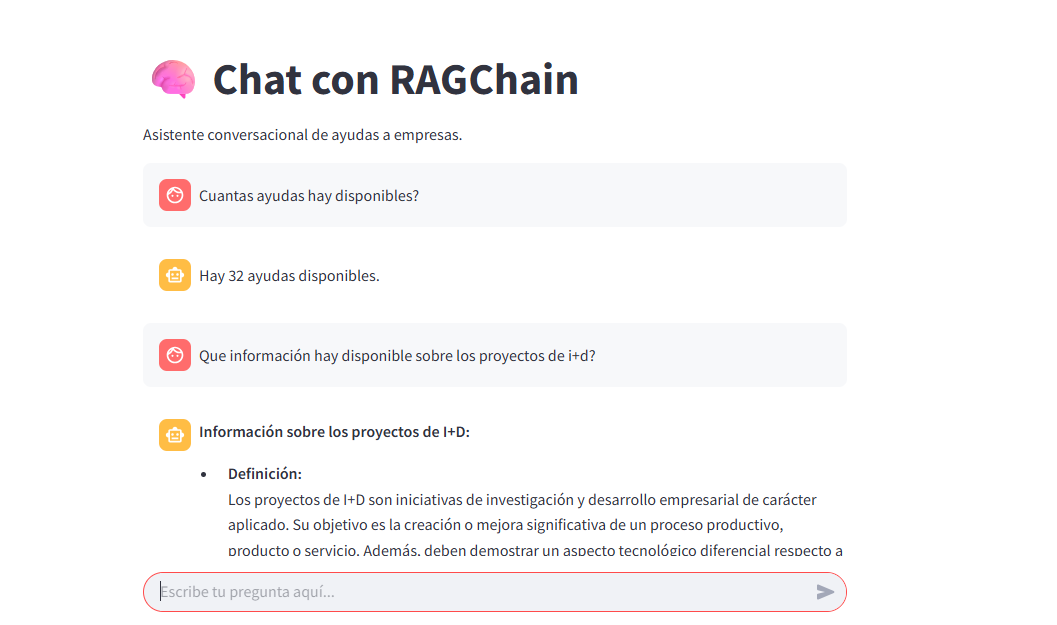
\includegraphics[width=0.8\textwidth]{figs/streamlit_app.png}
	\caption{Interfaz gráfica con Streamlit}
	\label{fig:context-anoni1}
\end{figure}

Finalmente, se implementa mediante Streamlit una interfaz gráfica sencilla a modo de chat, donde se pueden enviar mensajes directamente al sistema.
Streamlit permite generar con un único script de Python una aplicación grafica de manera rápida y sencilla, la cual puede ser posteriormente desplegada con rapidez.



\section{Resultados}

Tras la implementación de cad auno d elos módulos lo que obtenemos es una solución completa con las siguientes características:

\begin{itemize}
    \item Una aplicación de asistencia conversacional, donde conversas con una IA que tiene acceso tanto a los documentos asociados a las ayudas como a los datos estructurados generados por el procesamiento.
    \item Cuando el usuario realiza una consulta, el sistema decide internamente si el contexto que necesita lo extrae de la base de datos SQL o de la vectorial. En cada caso, realiza una búsqueda de información y en base a esos datos genera una respuesta.
    En el caso de que la consulta sea a la base de datos vectorial, el sistema te devuelve una lista de fuentes empleadas.
    \item El propio sistema integra las pipelines de extracción y procesamiento de datos, con los que se puede mantener actualizada la aplicación realizando ejecuciones de manera periódica.
    \item El sistema está construido con una arquitectura modular, por lo que se pueden integrar nuevas fuentes de datos (portales de ayudas) con facilidad.
\end{itemize}